\section{Results}
\label{sec:results}

\subsection{Most releases are silent}
\gap{Prose.} 79\% of releases do not oscillate (regime S1) \src{acoustics/m2\_report.md}.
\begin{figure}
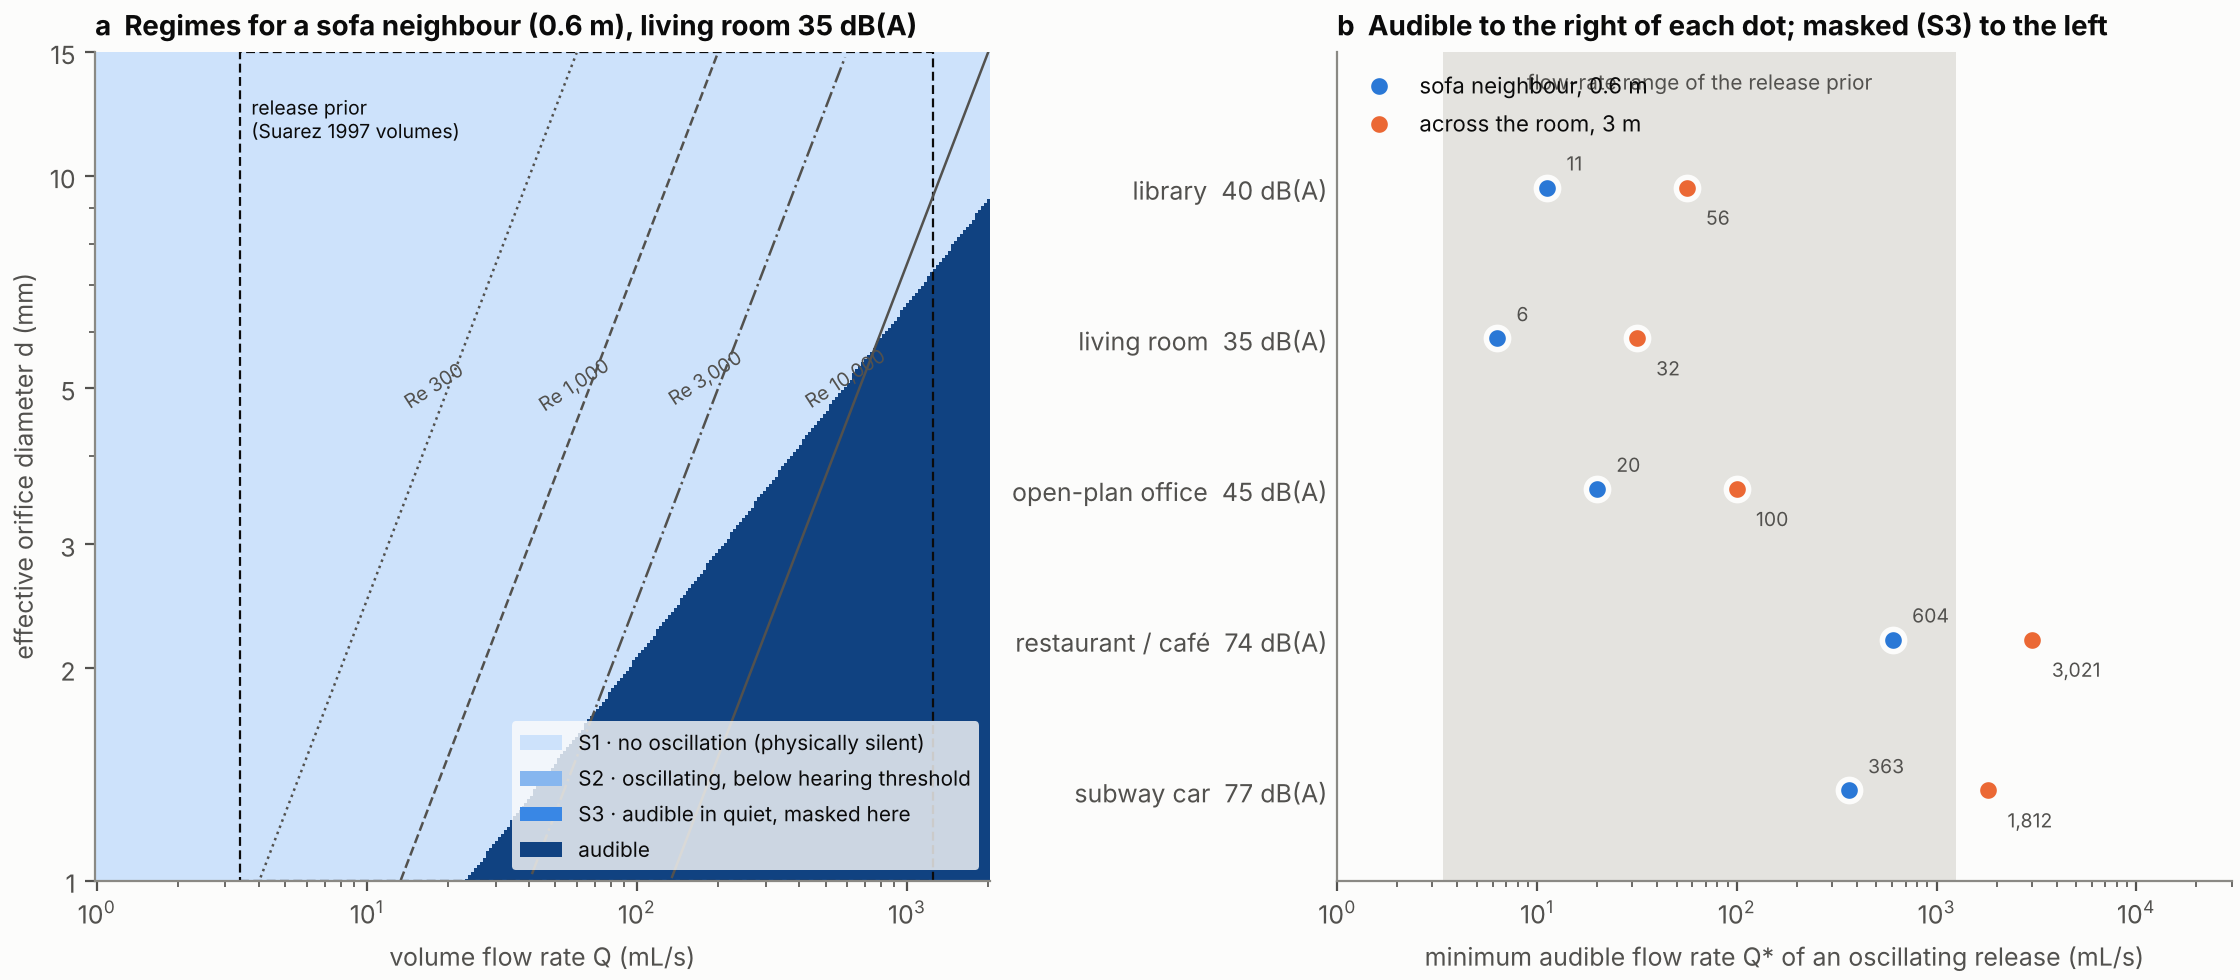
\includegraphics[width=\textwidth]{fig3_acoustic_regimes.png}
\caption{\gap{caption} Acoustic regimes.}
\label{fig:acoustics}
\end{figure}

\subsection{Validation}
\gap{Prose and merged figure (jet + CBL).}

\subsection{The physical ratio}
\gap{Prose.} Equal mass: $R$ = 1.35 (neighbour), 1.73 (own nose). As emitted: 0.92 (neighbour, $P(R>1)$ = 0.47), 1.15
(own nose). Sobol: release volumes explain about 0.6 of the variance as emitted \src{uq/m7\_report.md}.
\begin{figure}
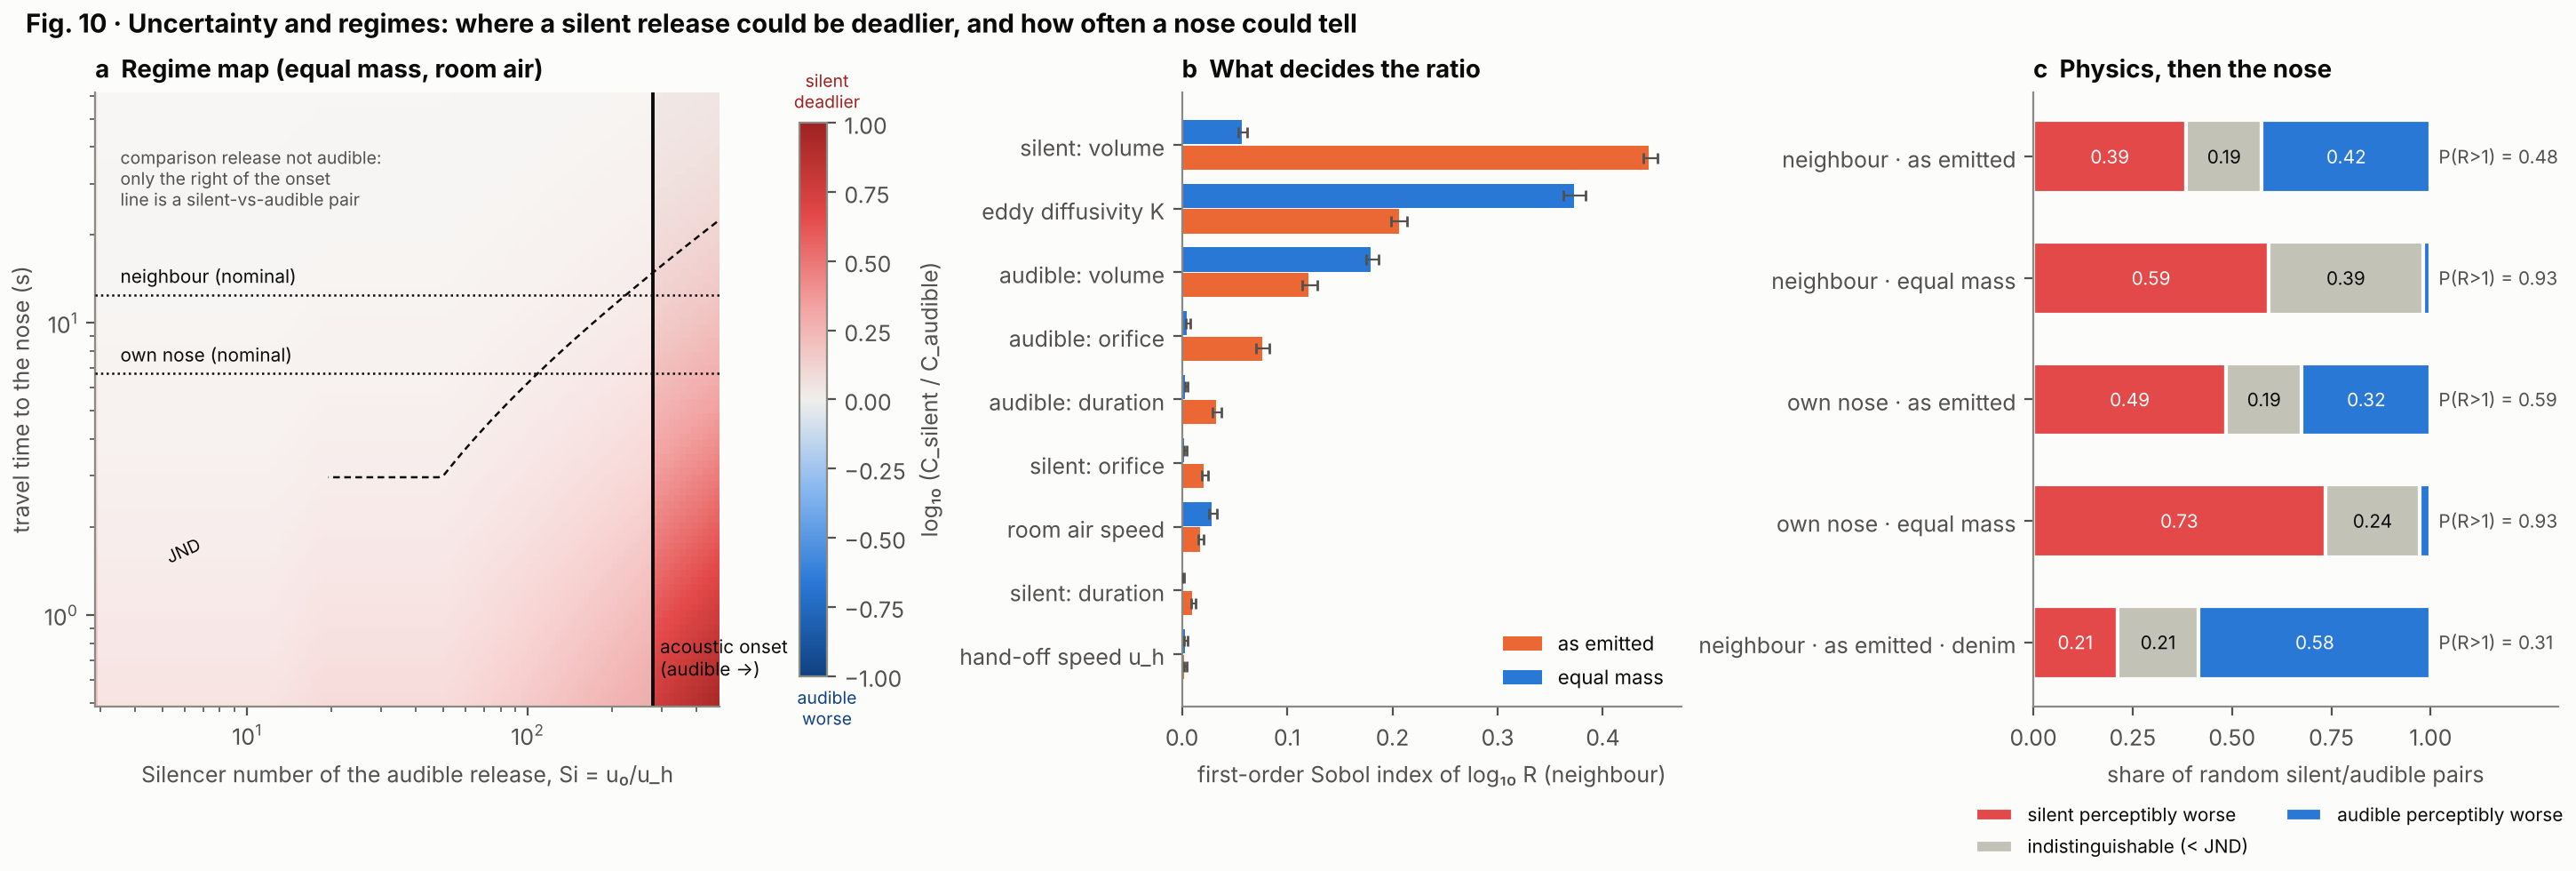
\includegraphics[width=\textwidth]{fig10_regime_uq.png}
\caption{\gap{caption} Regime map, first-order indices and the layered headline.}
\label{fig:uq}
\end{figure}

\subsection{A sofa}
\gap{Prose.} The backrest chimney carries the silent release over the releaser's head; the jet escapes it and reaches the
neighbour \src{cfd/cases/sofa/m4\_report.md}. With the releaser reclined by 4.5\,\textdegree, which closes the back
onto the backrest, the silent release leaves the seat-level wedge sideways and still rises behind the head. No
breathing zone receives a detectable dose. The audible jet now exceeds threshold at the releaser's own nose (OAV 2--4).
In both postures the breathing-zone ratio is $R \approx 10^{-11}$--$10^{-14}$ \src{cfd/cases/sofa/results\_rec4.5.json}.
\begin{figure}
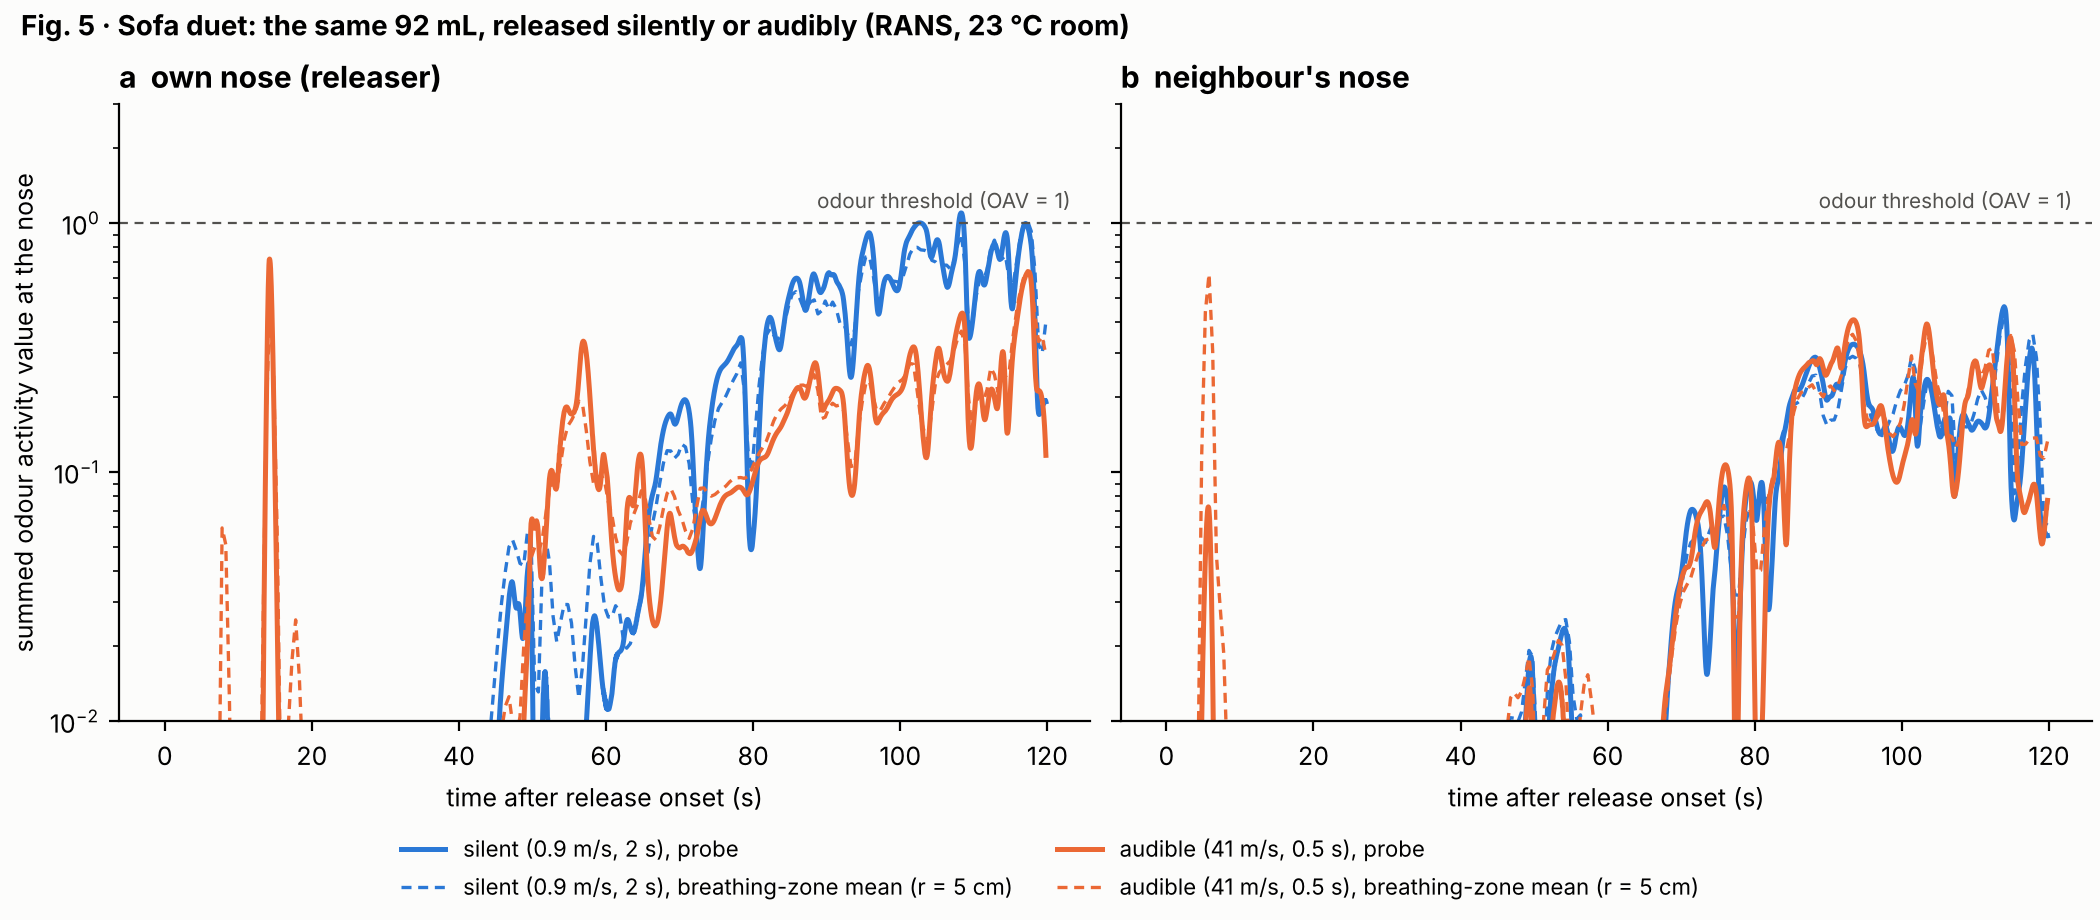
\includegraphics[width=\textwidth]{fig5_sofa_duet_noses.png}
\caption{\gap{caption} Sofa duet: nose time series.}
\label{fig:sofa}
\end{figure}

\subsection{Perception}
\gap{Prose.} Median silent/audible difference at the neighbour: 2.7\% in perceived intensity, below the JND
\src{perception/m6\_report.md}.

\subsection{The composition counter-argument}
\gap{Prose.} No link between passage volume and sulfur concentration; sulfur mass rises with volume
\cite{suarez1997}; nitrogen is blood-derived, not swallowed air \cite{levitt1970,tomlin1991}.

\subsection{Memory}
\gap{Prose.} Truth 0.49; bystander belief 0.67--0.92 across observer models; emitter unbiased
\src{perception/selection.json, uq/observer\_ps.json}.
\begin{figure}
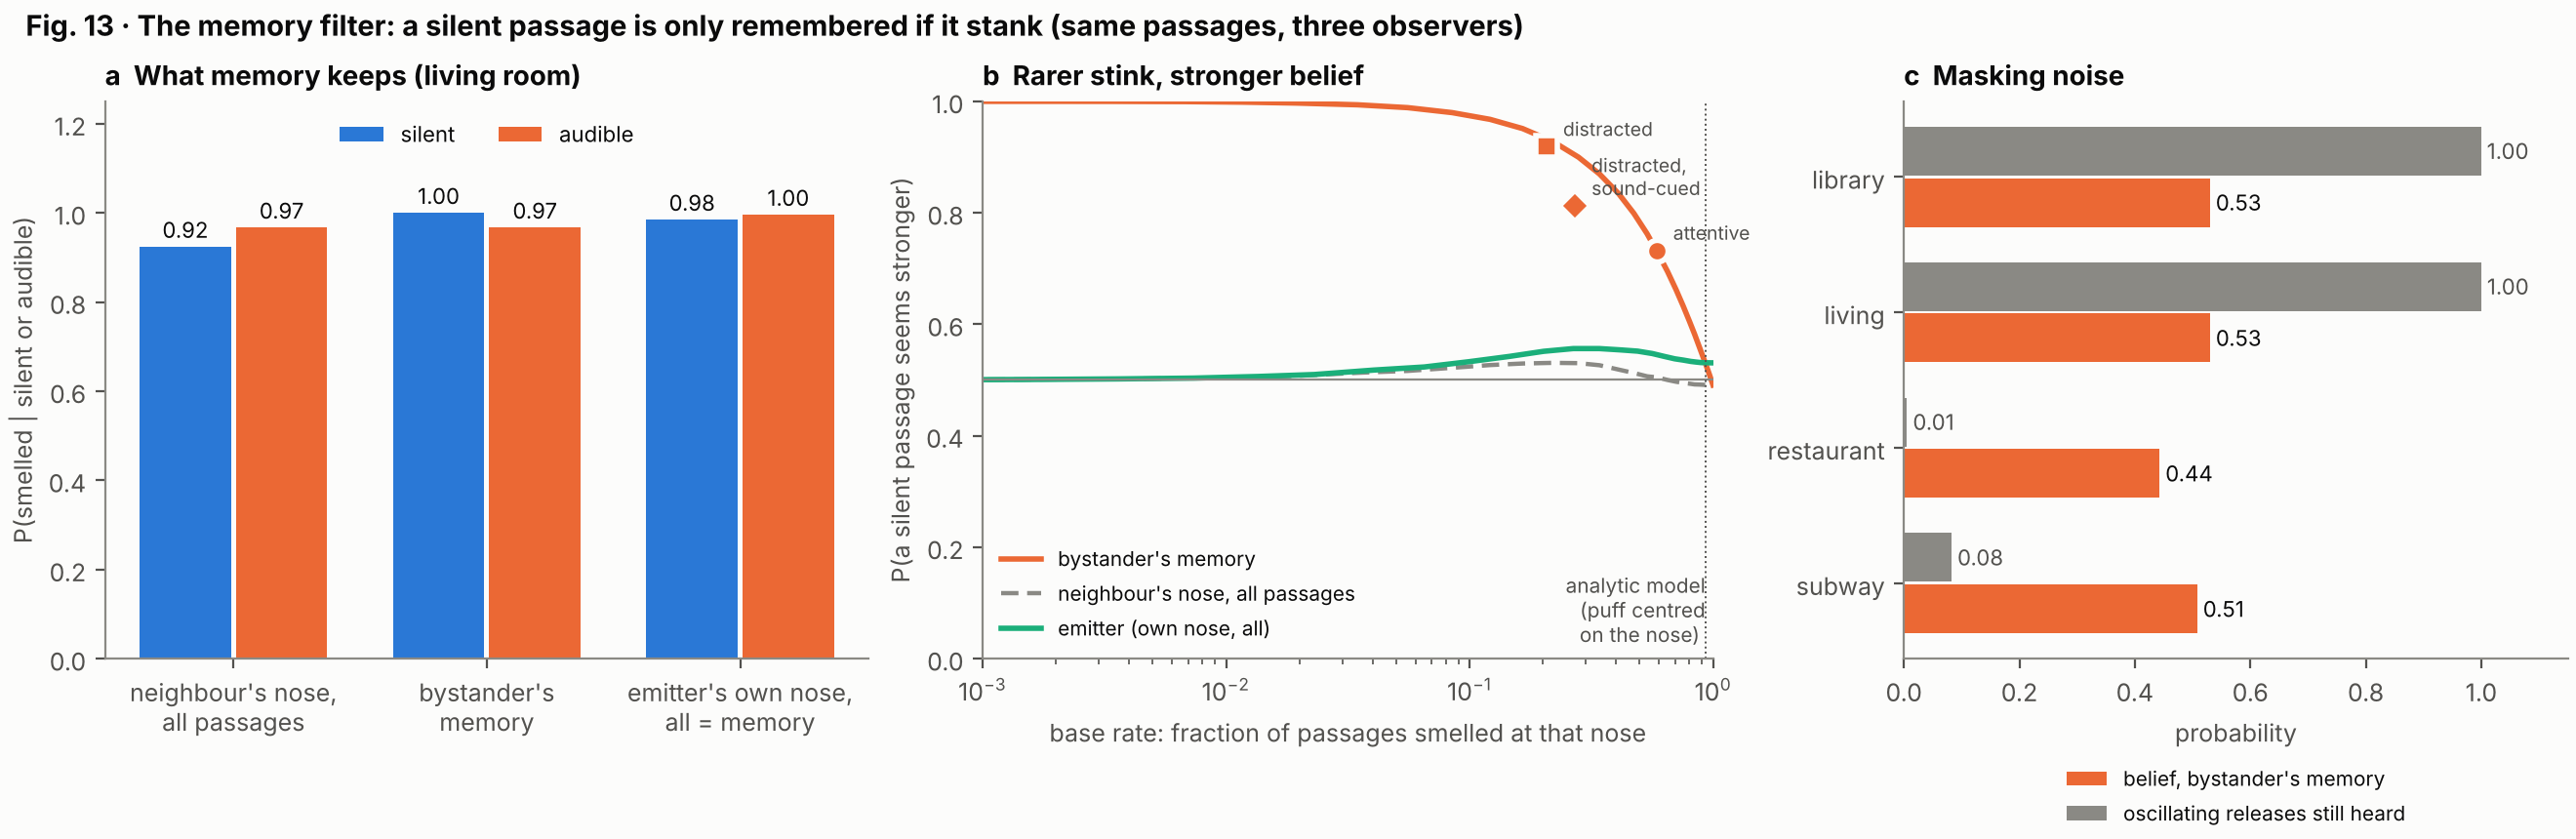
\includegraphics[width=\textwidth]{fig13_memory_filter.png}
\caption{\gap{caption} The memory filter.}
\label{fig:memory}
\end{figure}
